La crescente diffusione di dispositivi smart collegati tra di loro attraverso la rete secondo un meccanismo \verb+M2M+ (\textit{Machine to Machine}), denota un trend definito come \verb+IoT+ (\textit{Internet of Things}) \cite{Rfc7452}.

L'\verb+IoT+ rappresenta la più dirompente rivoluzione tecnologica della nostra vita.
Con un numero di \textit{device} connessi a Internet stimato tra i 50 e 100 miliardi entro il 2020, stiamo vivendo un cambiamento di paradigma in cui oggetti di uso quotidiano diventano interconnessi ed intelligenti \cite{IoT}.

Per questi dispositivi sono emerse differenti sfide:
\begin{itemize}
\item le connessioni devono avere un basso impatto sulle prestazioni del sistema, soprattutto considerando la scarsa potenza computazionale disponibile
\item la banda può essere limitata, non sempre disponibile o di scarsa qualità
\item le notifiche dovrebbero essere tempestive e causate da qualche evento
\end{itemize}

Con queste caratteristiche, è stato definito un nuovo protocollo \verb+MQTT+ (\textit{MQ Telemetry Transport}).
Nato nel 1999 da Andy Stanford-Clark di IBM e Arlen Nipper di Arcom, è diventato uno standard pubblico nel Marzo del 2013 sponsorizzato da IBM \cite{Mqtt}.
Si tratta di un protocollo di messaggistica estremamente semplice e leggero posizionato in cima allo stack \verb+TCP/IP+.
Una variante del protocollo, definita \verb+MQTT-SN+, è stata sviluppata per funzionare su reti non \verb+TCP/IP+ come \textit{ZigBee} \cite{MqttSn, ZigBee}.
Si basa sul pattern \textit{publish}/\textit{subscribe} (\textit{producer}/\textit{consumer}): comunicazione di messaggi tra diversi processi, oggetti o altri agenti.

Il funzionamento logico di una comunicazione si basa sul concetto di comunicazione asincrona tra due o più player, i quali dialogano attraverso un tramite (\textit{broker}).
Il \textit{publisher} di un messaggio (\textit{producer}) pubblica il proprio messaggio al \textit{broker}, potendo anche specificare il \textit{topic} del messaggio.
I \textit{subscriber} si rivolgono a loro volta al \textit{broker} abbonandosi nella ricezione di messaggi o solo di alcuni \textit{topics}.
Il \textit{broker} inoltra ogni messaggio inviato da un \textit{publisher} a tutti i \textit{subscriber} interessati a quel messaggio.
La connessione non viene necessariamente chiusa a messaggio ricevuto o inviato ed i partecipanti non devono richiedere nuovi messaggi ad intervalli di tempo, ma sono notificati immediatamente.

\begin{figure}[H]
  \centering
  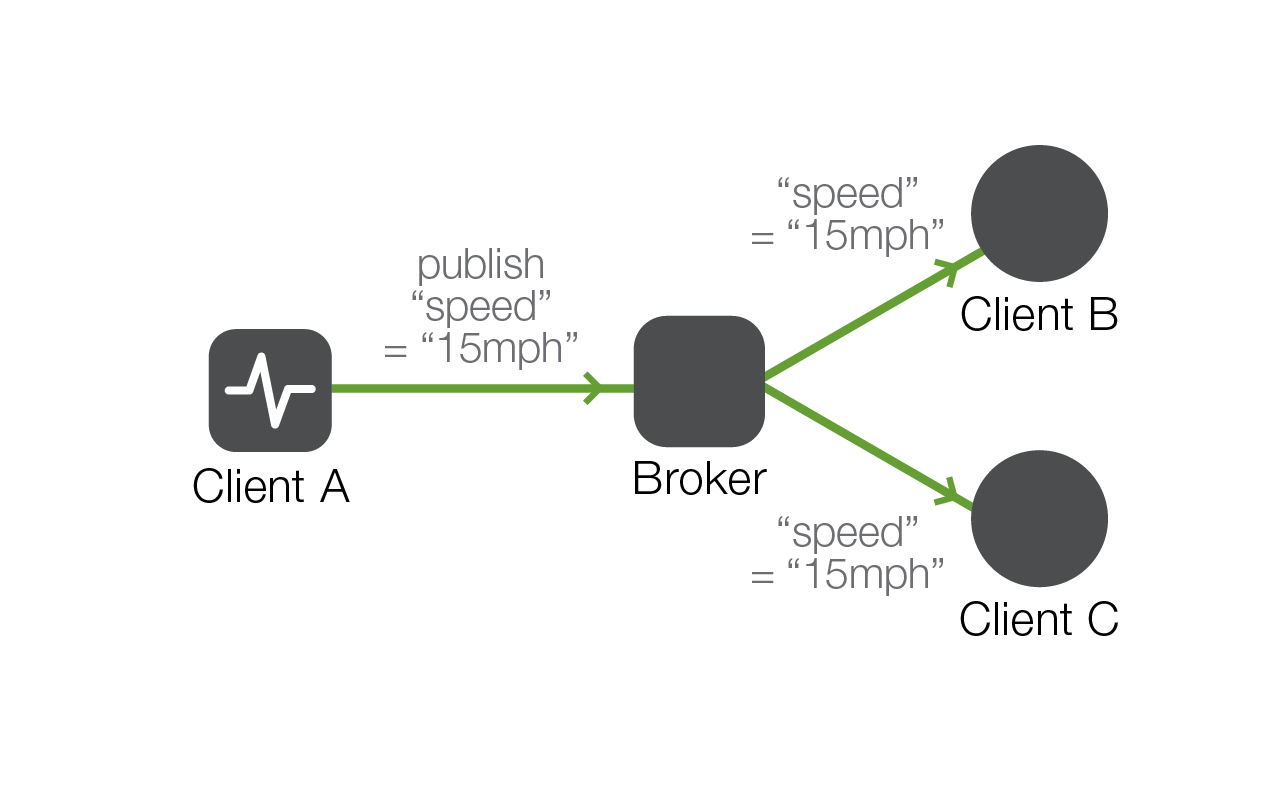
\includegraphics[width=0.95\linewidth, keepaspectratio]{mqtt}
  \caption{Modello del dispatch di un messaggio da parte del broker a diversi subscriber}
  \label{fig:mqtt}
\end{figure}

\subsection{QoS}
\label{sub:mqttQos}

\verb+MQTT+ fornisce la possibilità di garantire che il messaggio sia effettivamente stato consegnato attraverso un meccanismo denominato \verb+QoS+ (\textit{Quality of Service}).
Con l'ipotesi che la banda può essere limitata o inaffidabile, i \textit{client} possono negoziare il giusto livello di qualità del servizio in base alle loro esigenze:
\begin{description}
\item[QoS 0 – at most once] il messaggio non deve essere ammesso dal destinatario o salvato e rinviato dal mittente (stessa garanzia prevista dal protocollo \verb+TCP+)
\item[QoS 1 – at least once] viene garantito che il messaggio sia stato consegnato almeno una volta ed è possibile che lo stesso messaggio venga recapitato più volte
\item[QoS 2 - exactly once] viene garantito che il messaggio verrà consegnato esattamente una volta
\end{description}

\begin{figure}[H]
  \centering
  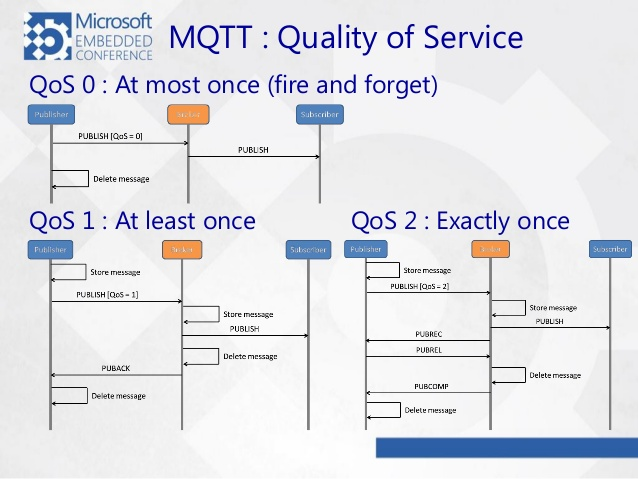
\includegraphics[width=0.95\linewidth, keepaspectratio]{qos}
  \caption{I vari livelli di qualità del servizio disponibili tramite MQTT}
  \label{fig:qos}
\end{figure}
